\section{Running a Kernel}
To run a kernel, the host program executes the \verb/run_kernel/ function with a reference to the kernel address, as well as the number of threads it wants to spawn.
Listing \ref{lst:run-kernel} shows the code required for running a kernel.

\begin{c-code}[caption=Running a kernel, label=lst:run-kernel]
run_kernel(fill_screen, 4096);
\end{c-code}

\begin{figure}[H]
    \centering
    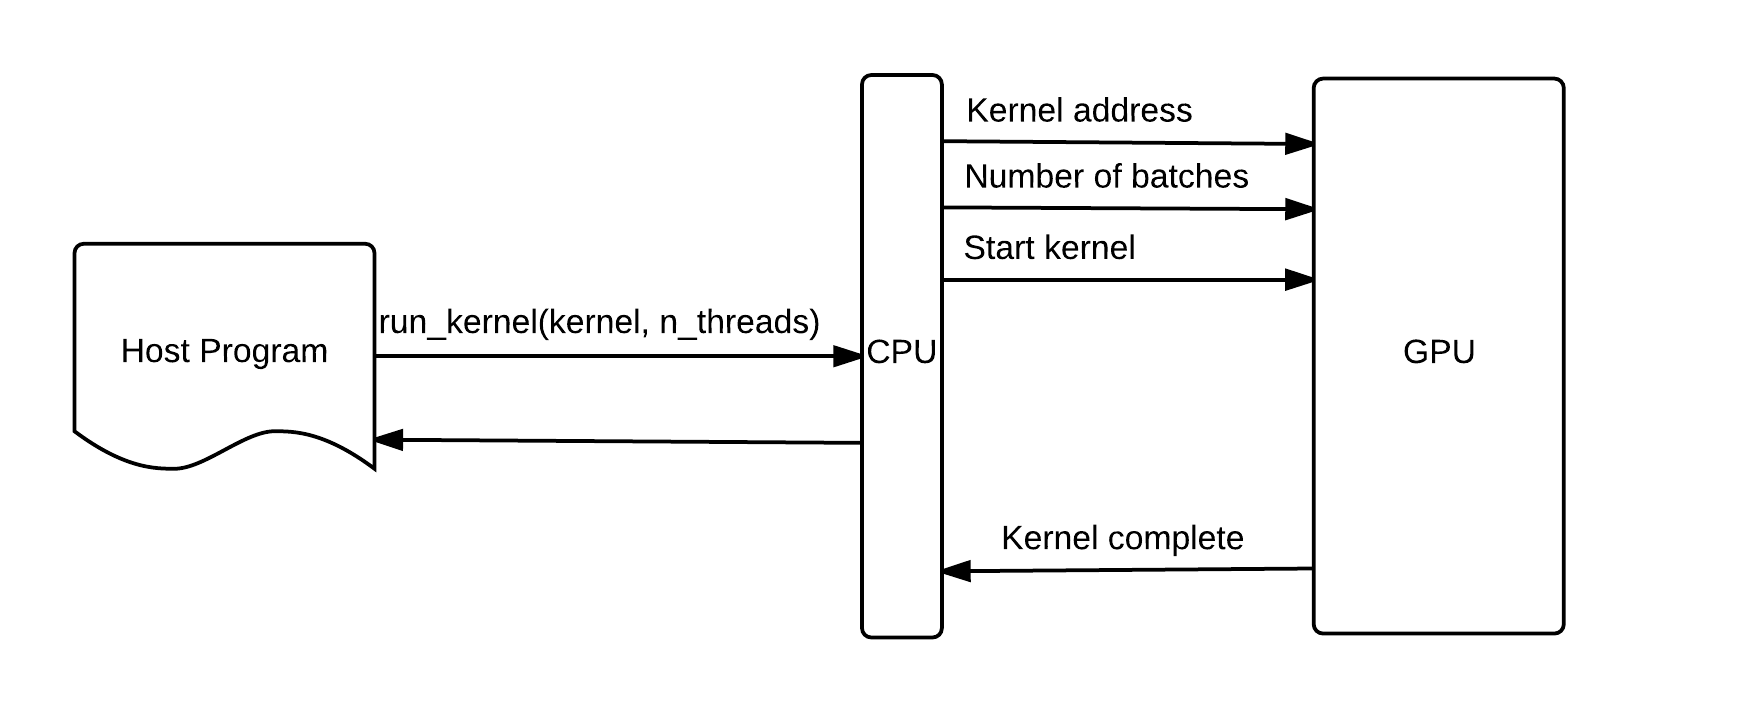
\includegraphics[width=\textwidth]{../cpu/diagrams/running_a_kernel.png}
    \caption{Starting a kernel on the GPU.}
    \label{fig:running_a_kernel}
\end{figure}

To tell the GPU to start executing a kernel,
there are two pieces of information the GPU needs.
Which kernel should be started, and how many threads should be executed.
As can be seen in figure \ref{fig:memory_map}, there exists a dedicated address space for starting kernels.
It is the same size as the instruction memory,
meaning any valid instruction address will be valid also in the \emph{start kernel} space.
Writing to the instruction address,
but in the \emph{start kernel} space instead of the instruciton memory will tell the GPU to start executing from that particular instruction.

When writing to this \emph{start kernel} address, we use the data value for telling the GPU how many threads should be spawned.
For example, say the \verb/fill_kernel/ reference points to instruction 100 in instruction memory.
Then, executing the code in listing \ref{lst:run-kernel} will write the value 4096 to address 100.

To increase the maximum number of threads which may theoretically be spawned,
the number of \emph{batches} of threads is what is actually written.
A batch represents the nuber of threads which can be executed at the same time,
and will be explained in more detail in the next chapter. \todo{will it?}
The number of threads in a batch will typically be between 8 and 32 depending on the size of the GPU.
What's important is that this work-around will help in increasing the number of threads that can be spawned from 2\textsuperscript{16} up to 2\textsuperscript{21},
which is needed for the target resolution of 512*256, i.e. 2\textsuperscript{17} pixels.

Only one kernel can execute at the time in the GPU.
Because of this, the \verb/run_kernel/ call is designed to block until the kernel has completed execution.
This is implemented by having a dedicated line from the GPU to the CPU which will be asserted whenever the GPU is idle.
The CPU may sleep when the GPU is executing and wait for an interrupt on this line.
